\documentclass[]{article}

\usepackage{graphicx}
\usepackage{float}
%opening
\title{Olin Computational Robotics Warmup Project}
\author{Dhasharath Shrivathsa}

\begin{document}

\maketitle

\begin{abstract}
Submission and writeup for the Spring 2017 Warmup project, consisting of a Neato performing:
\begin{itemize}
	\item Go in a square
	\item Follow a wall
	\item Follow a person
	\item Obstacle avoidance
\end{itemize}
\end{abstract}
\section{Tasks}
\subsection{Square}
I accomplished the task of going in a square by focusing on the \verb$\odom$ frame, which provides odometry from the neato's wheel encoders. THe algorith used is very simple, with a finite state machine providing all control. It takes a single parameter, the length of the sqaure, called distance in the FSM.
\begin{figure}[H]
	\centering
	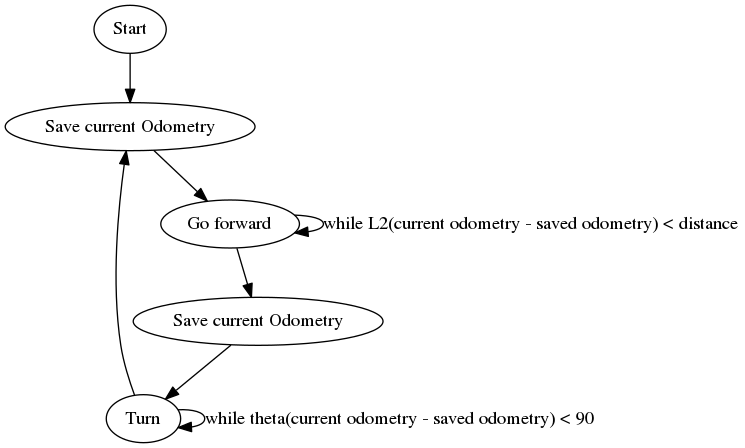
\includegraphics[width=0.7\linewidth]{square}
	\caption{Square FSM}
	\label{fig:square}
\end{figure}

\subsection{Wall follower}
The wall follwer uses RANSAC with a linear model to solve the equation fo a line in the cartesian \verb|\odom| frame, then line follw a parallell line. 
The FSM looks like
\begin{figure}[H]
	\centering
	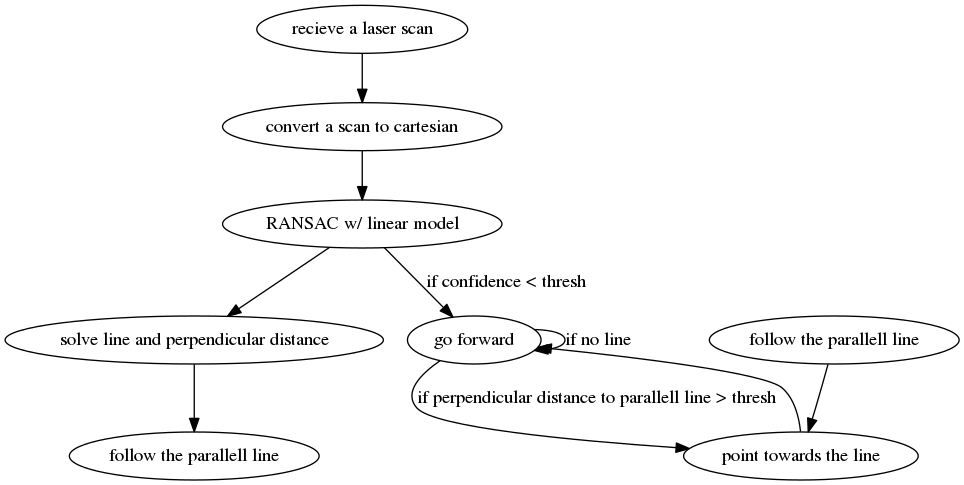
\includegraphics[width=0.7\linewidth]{wall_follower}
	\caption{Wall follower FSM}
	\label{fig:wallfollower}
\end{figure}
\subsection{Person follower}
Person following can be decomposed into two tasks, person localization and object avoidance (see next section).

Recognizing a person from a laser scan is \textit{really hard}, so we can focus on a more general problem, that of movement detection. If we compare two laser scans (aligned with Iterated closest point, a point set registration algorithm that results in an optimal affine transform) from successive times, and calculate the L2-norm for each point in the new point cloud to it's closest point in the old, shifted set. If there are points with large euclidian distances, that signifies movement.


We can detect the mask of the points that denote movement with a $k$-means cluster with \verb|n_clusters=2|, to form disjoint subsets of the newest pointcloud based off point shift. We can then navigate to the centroid of the points in the movement subset.

\subsection{Object avoidance}
Object avoidance with a goal can be handled by designing a cost function that weights each point as the inverse squared euclidian distance, and the distance from the goal with euclidean L2 distance. This lets us calcuate the Hessian and Jacobian, and greedliy go in the direction of max slope.
\section{Programming style}
\subsection{ROS wrapper}
I wrote a ROS wrapper so that I can just run a plain \verb|.py| file that takes care of all the \verb|roslaunch/rosrun| under-the-hood machinery. This also sets up some of the boilerplate, like the call to \verb|init_node| and sets up a \verb|tf.TransformListener|.
\subsection{Neato wrapper}
The neato wrapper allows me to use python function calls for stuff like move primitives and base publisher and subscriber setup. This also lets me build data structures around historical laser scans and positions so that I can use those at later times, as well as log the current ones so that i can use it in a logic block
\subsection{Task-specific structure}
With the preceding structure, I can just subclass \verb|Neato| and implement the abstract \verb|logic| class that sits in the main loop to do all calculation and actual robot  logic. This means I can just write the logic implementation and all helper functions, using the provided OO-type wrappers by the superclasses for easy development.
\section{Challenges}
A challenge faced was getting the point sets to register in the person-following task. Iterated closest point is an optimized affine transform to map one pointcloud onto another, but only non-python implementations exist. For my learning goals, I wrote an implementation of it in python. It's not very theoretically complex since it's just an optimum affine transform, but it's implementation is pretty interesting
\section{Improvments}
If I was to improve this further, I'd do total path plannning so that the obstacle avoider doesn't get trapped in local minima. This is pretty easy to implement.
\end{document}
